%intro to seqence analysis, sessions
Magnitude analysis and categorization are both appropriate for answering research questions that are simply manifested in the IDE data stream. However, a more powerful way of analyzing activity logs is through sequence analysis, which first breaks activity sequences into session, according to some criteria, and then reports upon characteristics of that session. 

A session is a particular interaction with an IDE by a specific user in order to complete a task (e.g. refactoring, looking for a starting point for a maintenance task, etc.), consisting of all of IDE events in a given time span.
For instance, answering the research question of ``Are developers successful at finding initial points in the code for a software maintenance task?'' requires that the sequence of IDE events corresponding to each maintenance task be identified, before we can perform further analysis using either magnitude or categorization analysis. The granularity of a session is determined by the guiding research question. For certain research questions, we may be interested in a smaller session (e.g. searching the code base), while for others we may need to consider a longer time span (e.g. performing a maintenance task, developing a new feature). 

%how difficult or easy is it to determine sessions
In many cases, extracting sessions from activity sequences can be challenging as it impossible to know exactly when a developer begins or ends a particular task, without understanding his or her underlying thought process. There are several possibilities in how session extraction can be performed, based on the task related to the specific research question. One possibility is to use sentinels, which are specific actions where we can detect a task begins or ends. For instance, in code search, submitting a query to the code searcht tool begin one task and end the prior task in the activity stream. Another possibility is to use the passage of time to extract sessions, where time without any activity is used as a signal of task start or finish. Coman et al.'s \cite{Coman-TaskIdent} algorithm uses a combination of key events in the activity stream and time distance between such events to extract relevant sessions corresponding to developer tasks. In lab validation studies this algorithm has shown very high accuracy (80\%) when compared to the ground truth reported by developers, however this accuracy may not hold up in an industrial setting\cite{Zou-ComanIndustry}.


%example
As an example of sequnce analysis, consider a researcher investigating finding initial points in the code for a software maintenance task. Specifically, the developer is interested in the following research question ``Are users satisfied with file search results?''. This question, while impossible to answer via simple magnitude analysis can be investigated via session analysis. Using assumptions from in-lab studies that show that opening a search result followed by a long pause correlates with user satisfaction we can analyze activitiy logs to determine how often user behavior indicated satisfaction in the field. The researcher may break activity logs into sessions, starting with a search being executed and ending on the last interaction with that result set. He could calculate additional characteristics from this raw data, such as the amount of time spent per session, the number of results reviewed, and the number of files opened.   


%\begin{figure*}[t]
%\centering
%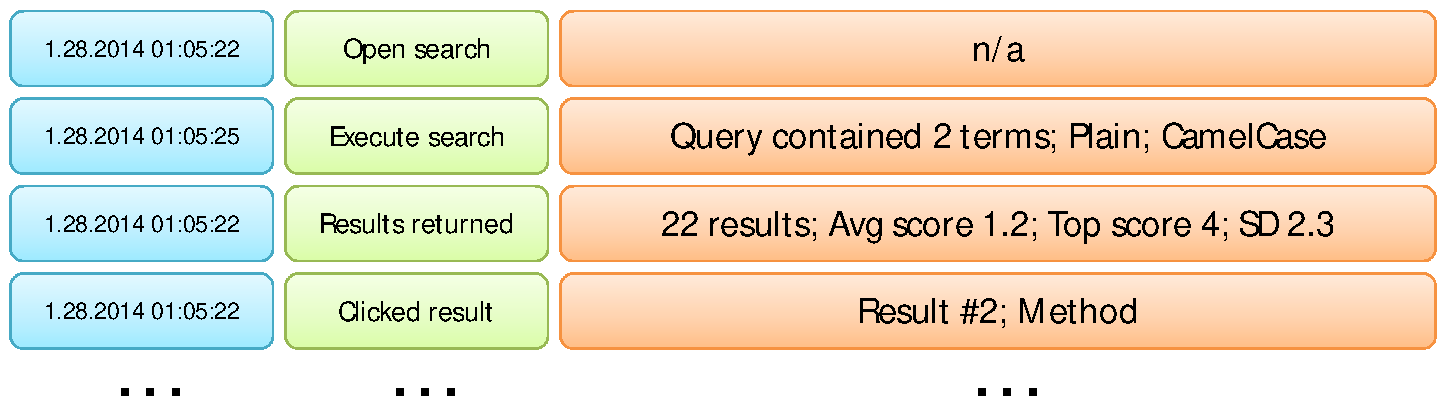
\includegraphics[width=1\columnwidth]{../Graphics/activityLogActual.pdf}
%\caption{Pairwise matches across categories, including matching and mismatching pairs.}
%\label{fig:actual}
%\end{figure*}

%Sequence analysis is currently the most powerful tool we have for analyzing logs. While there has been preliminary work to complete annotate activity logs into tasks or even states (e.g., editing, searching, navigating, testing, etc.) these analyses are currently unreliable. In fact, we believe that because user behavior is often multi-purposed there will remain major obstacles to inferring higher-level user states from activity streams, ultimately limiting the usefulness of any full log analysis. 

